\section{Regulární grafy}
\df {\it \emph{Regulární graf} je graf, jehož všechny vrcholy mají stejný stupeň. Graf je $k$\emph{-regulární}, je-li stupeň všech jeho vrcholů $k$.}

\begin{itemize*}
\item 0-regulární grafy se skládají z izolovaných vrcholů
\item 1-regulární grafy jsou disjunktním sjednocením hran
\item 2-regulární grafy jsou disjunktním sjednocením cyklů a nekonečných cest
\item 3-regulární grafy nazýváme kubické, patří mezi ně např. Petersen
\end{itemize*}

\vt (o vlastních číslech) {\it Graf $G$ je $k$-regulární $\Leftrightarrow$ matice sousednosti $G$ má vlastní číslo $k$ a odpovídající vlastní vektor $(1,\dots,1).$ 
$k$-regulární graf je souvislý $\Leftrightarrow$ vlastní číslo $k$ má násobnost 1.}

\subsection{Silně regulární grafy}
\df {\it \emph{Silně regulární graf} je $d$-regulární, $\forall$ hranu $xy\in E$ $\exists!e$ vrcholů $u: ux,uy\in E$ a $\forall$ nehranu $xy\not\in E$ $\exists!f$ vrcholů $u: ux,uy\in E$.}

Abychom mohli zanedbat triviální případy, dodáváme $f>0$ a $G\neq K_n$.
Příkladem silně regulárního grafu je úplný bipartitní graf se stejně velkými
partitami ($e=0$). Nejmenším nebipartitním silně regulárním grafem je
pěticyklus ($e=0$, $f=1$). Nejmenší graf, který je regulární, ale není silně
regulární je šesticyklus.

\vt (Friendship theorem) {\it Nechť $G=(V,E)$ je graf, že každé dva vrcholy $u,v$ mají právě jednoho společného souseda. Pak existuje $u$, že $\deg(u) = n-1$.}

Neboli Friendship theorem tvrdí, že takový silně regulární graf musí vypadat jako
mlýn (hromádka trojúhelníků, které se stýkají v jednom centrálním vrcholu).

\subsection{Moorovy grafy}

Moorovy grafy jsou $r$-regulární grafy bez krátkých cyklů (délky 3 a 4) s nejmenším možným počtem vrcholů. Obecně se definují i pro jiný girth (délku nejkratší kružnice), definice z LAKu je následující:

\df Moorův graf je takový $r$-regulární graf bez troj- a čtyř-úhelníků, kde $|V| = 1 + r + r(r-1) = r^2 + 1$.

Konstrukcí lze ukázat, že menší počet vrcholů už implikuje malý cyklus, nebo rozbije $r$-regulárnost.

\vt Moorův graf existuje pro $r=1,2,3,7$, pro $r=57$ se neví (otevřený problém) a pro žádné další $r$ neexistuje.

\dk (Idea) Mějme graf $G$ Moorův a $A$ jeho matici sousednosti. Zapišme druhou 
mocninu $A$ jako stupeň na diagonále a prohozené 0 a 1 jinde a upravme:
\begin{align}
	&A^2 = r\In + ({\bf J}_n- A - \In) \\
	\label{moorova-matice}&A^2 + A + (1-r)\In = {\bf J}_n
\end{align}
Dále pro nějaké $\lambda\in \Sp(A)$ a $x$ odpovídající vlastní vektor:
\begin{align}
	\label{moorova-mocnina}A^2 x = AAx = A\lambda x = \lambda A x = \lambda 
	\lambda x = \lambda^2 x
\end{align}
A dosadíme (\ref{moorova-matice}) za $A$:
\begin{align}
	{\bf J}_nx = (A^2 + A + (1-r)\In)x = (\lambda^2 + \lambda + (1-r))x
\end{align}
A tedy $(\lambda^2 + \lambda + 1 -r) \in \Sp({\bf J}_n)$. Vlastní čísla matice ${\bf J}_n$ 
(matice samých jedniček) ale známe, jsou to $\{0^{(n-1)}, n^{(1)}\}$. Zjevně pro 
$\lambda = r$ vyjde vlastní číslo $n$, je tedy potřeba vyřešit kvadratickou 
rovnici s parametrem $r$:
\begin{align}
	\lambda^2 + \lambda + 1 - r = 0
\end{align}
Jak na to půjdeme? Vyjádříme si $\lambda$ známým vzorečkem pro kořeny:\footnote{$D=b^2-4ac,\quad x_{1,2} = {-b \pm \sqrt D \over 2a}$}
\begin{align}
	\lambda_{1,2} = \frac{-1\pm \sqrt{1-4(1-r)}}{2} = \frac{-1\pm\sqrt{4r-3}}{2}
\end{align}
Násobnost označíme $m_1, m_2$. Stopa matice je suma vlastních čísel včetně
násobností, ale také součet čísel na diagonále. Protože matice sousednosti $A$
má na diagonále vždy nuly, platí rovnice:


\begin{align}
	\Tr(A) = r+m_1\lambda_1 + m_2\lambda_2 = 0
\end{align}
Nejdříve
upravíme do formy (násobení dvěma a přeskupení):
\begin{align}
	2r - \sqrt{4r-3}(m_1-m_2) - \underbrace{(m_1+m_2)}_{m_1+m_2=n-1=r^2} &= 0\\
	2r - r^2 + \sqrt{4r-3}(m_1 - m_2) &= 0 
	\label{4-2:rovnice}
\end{align}
Moorův graf je $r$-regulární, $r\in\N$, tedy máme dvě možnosti:
\begin{enumerate}
	\item $\sqrt{4r-3} \not\in \Q$: potom $m_1 = m_2$ a tedy $r = 2$.
	\item $\sqrt{4r-3} = s \in \Q$, což implikuje\footnote{Odmocnina z celého čísla je
  vždy celé číslo či iracionální číslo, nikdy zlomek.} $s \in \N$.
  Substitucí $4r - 3 = s^2$ do rovnice \ref{4-2:rovnice} získáme
	$s \in \set{1, 3, 5, 15}$, což dává $r \in \set{1, 3, 7, 57}$.
\end{enumerate}
\qed


\subsection{Regularita a Hamiltonovskost}
\vt (Dirac) {\it Máme-li souvislý graf $G$, $n \ge 3$ a stupeň každého vrcholu je alespoň $n\over 2$, pak je $G$ hamiltonovský.} 

Důkaz vezme nejdelší cestu v $G$ a hledá se spor s tím, že je nejdelší. Diracovu větu použijeme v důkazu následující věty od Nash-Williamse. 

\vt (Nash-Williams) {\it Každý $k$-regulární graf na $2k+1$ vrcholech obsahuje Hamiltonovskou kružnici.}

\dk Mějme $k$-regulární graf $G$ na $2k+1$ vrcholech. Přidáme k němu nový vrchol $w$ a spojíme ho se všemi vrcholy $G$. Výsledný graf $H$ má $2k+2$ vrcholů s minimálním stupněm $k+1$. Dle Diracovy věty je $H$ Hamiltonovský. Odebráním $w$ z $H$ získáme v $G$ Hamiltonovskou cestu $v_0v_1\dots v_{2k}$.

\begin{wrapfigure}{R}{6cm}
\centering
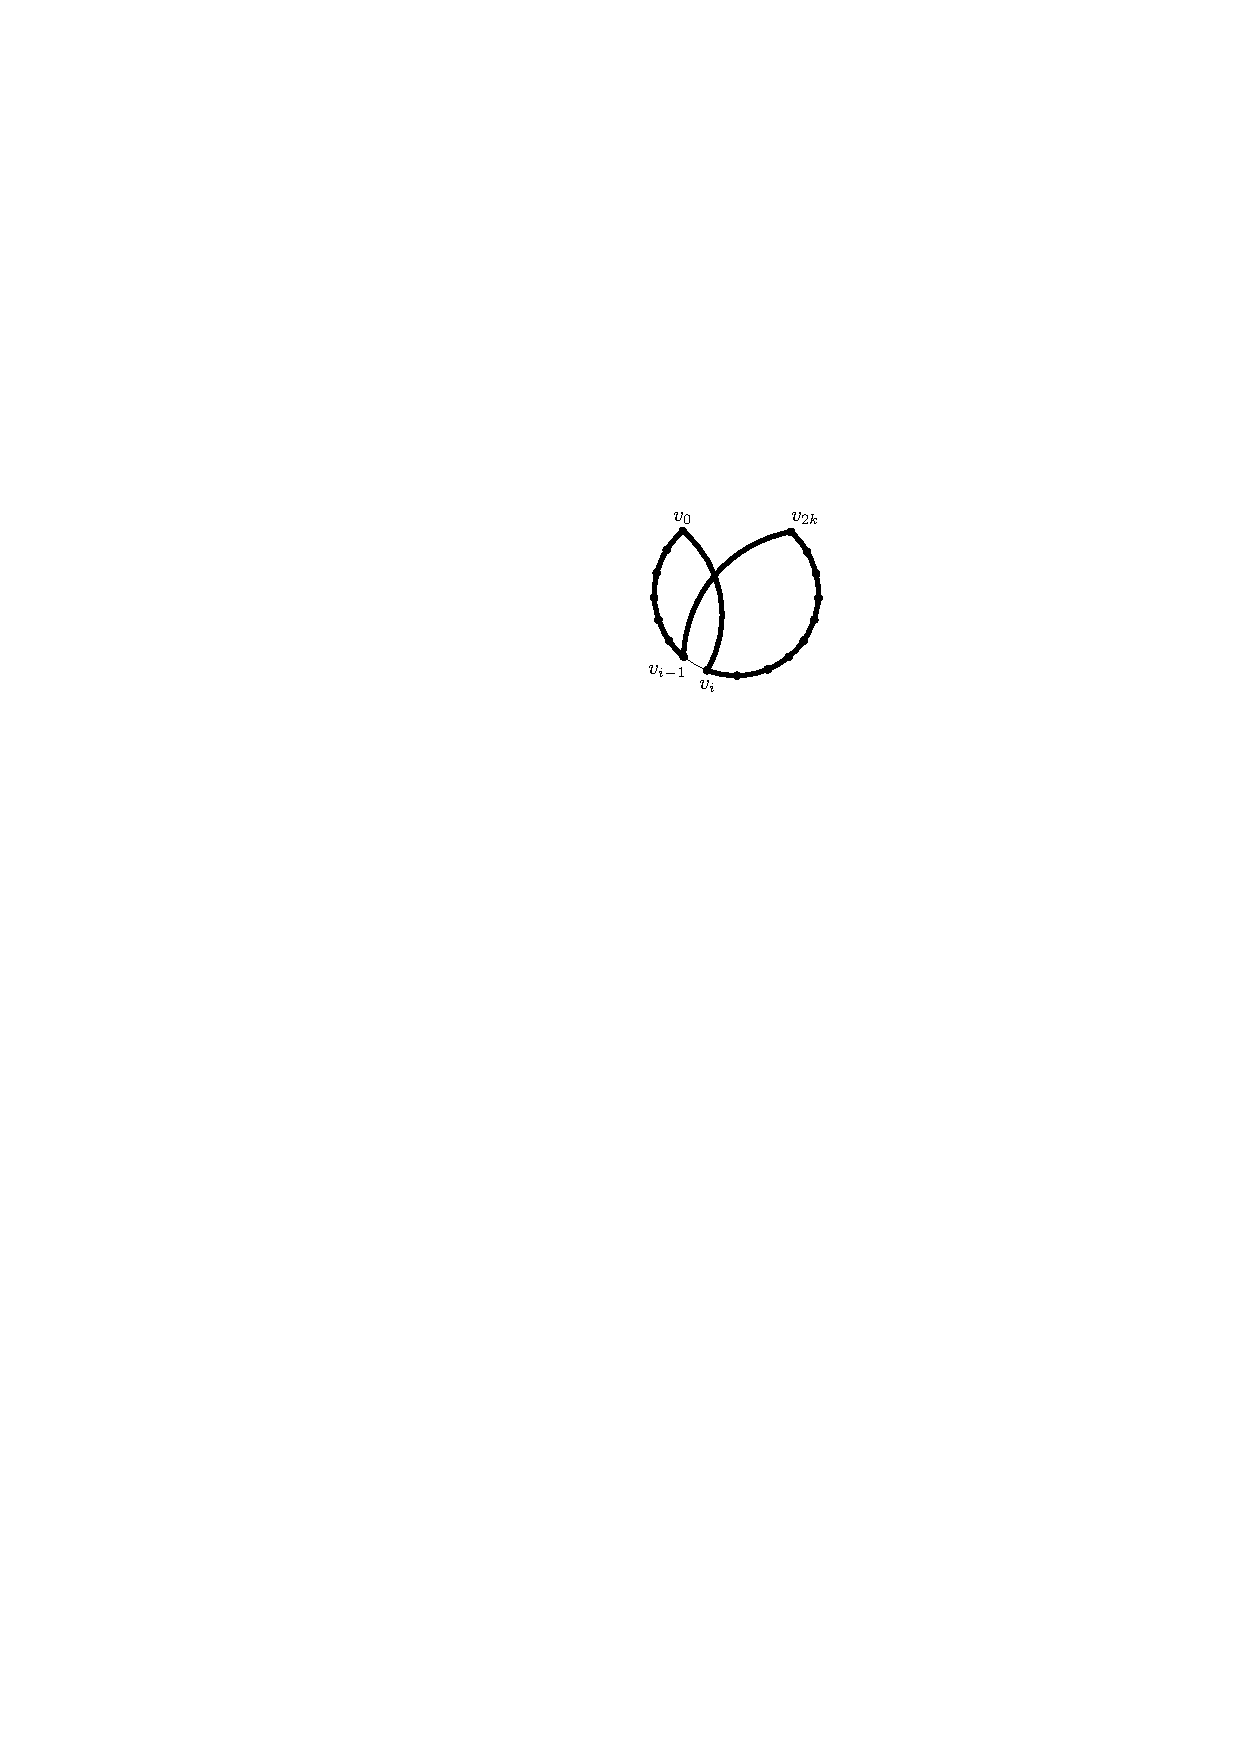
\includegraphics[width=5cm]{img/nash-williams4.pdf}
\caption{Triviální případ}
\label{dk:nw-triv}
\end{wrapfigure}

Předpokládejme že neexistuje dvojice na sousedních vrcholů $v_{i-1}v_i$, přes které by šla uzavřít kružnice (viz Obrázek \ref{dk:nw-triv}). Pak ale nutně platí, že když $v_0v_i \in E$, pak $v_{i-1}v_{2k} \not\in E$. Vrchol $v_{2k}$ má $k$ sousedů, ale nesmí mezi nimi být žádné vrcholy, jejihž pravý soused je spojen s $v_0$. Jinými slovy, $v_0$ nám vyblokuje $k$ vrcholů, do kterých nesmí vést hrana z $v_{2k}$ a ten sousedí se všemi ostatními. Tedy, když $v_0v_i \not\in E$, pak $v_{i-1}v_{2k} \in E$ (tuto vlastnost použijeme později).

\textbf{Případ (i)} $v_0$ sousedí právě s vrcholy v první polovině cesty a $v_{2k}$ právě s vrcholy v druhé polovině cesty. Pak musí existovat dvojice vrcholů $v_i,v_j$ v první polovině cesty, mezi kterými nevede hrana. Kdyby vedla hrana mezi každými dvěma vrcholy v první polovině cesty, pak by byl stupeň $v_k$ vyšší, než $k$. Protože stupeň $v_i$ je $k$, existuje $v_l$ v druhé polovině cesty tž. $v_iv_l \in E$. Pak najdu HK (viz Obrázek \ref{dk:nw-i}).

\textbf{Případ (ii)} Existuje vrchol $v_i$ takový, že $v_{i+1}v_0 \in E$, $v_iv_0 \not\in E$. Pak podle vlastnosti dokázané výše je $v_{i-1}v_{2k} \in E$. Potom $G$ obsahuje $2k$-cyklus $v_{i-1}v_{i-2}\dots v_0v_{i+1}\dots v_{2k}$ (viz Obrázek \ref{dk:nw-ii}). Přejmenujme $2k$-cyklus $C$ na $u_1u_2\dots u_{2k}$ a $u_0$ bude vrchol $G$, který v $C$ není. Potom $u_0$ nemůže sousedit se dvěma sousedními vrcholy $C$ (jinak by existovala HK) a tedy sousedí s každým druhým vrcholem $C$, řekněme s $u_1, u_3, \dots, u_{2k-1}$. Nahrazením $u_{2j}$ za $u_0$ ($\forall j$) dostaneme jiný maximální cyklus v $G$ a tedy $u_{2j}$ musí mít sousedy $u_1, u_3, \dots, u_{2k-1}$ (stejný argument jako v předchozí větě). Pak ale $u_1$ musí sousedit s $u_0, u_2, \dots, u_{2k}$ a tedy $\deg u_1 \ge k+1$, což je spor s $k$-regularitou. Tudíž je $G$ Hamiltonovský.
\qed

\begin{figure}[h]
\centering
\begin{subfigure}{7.5cm}
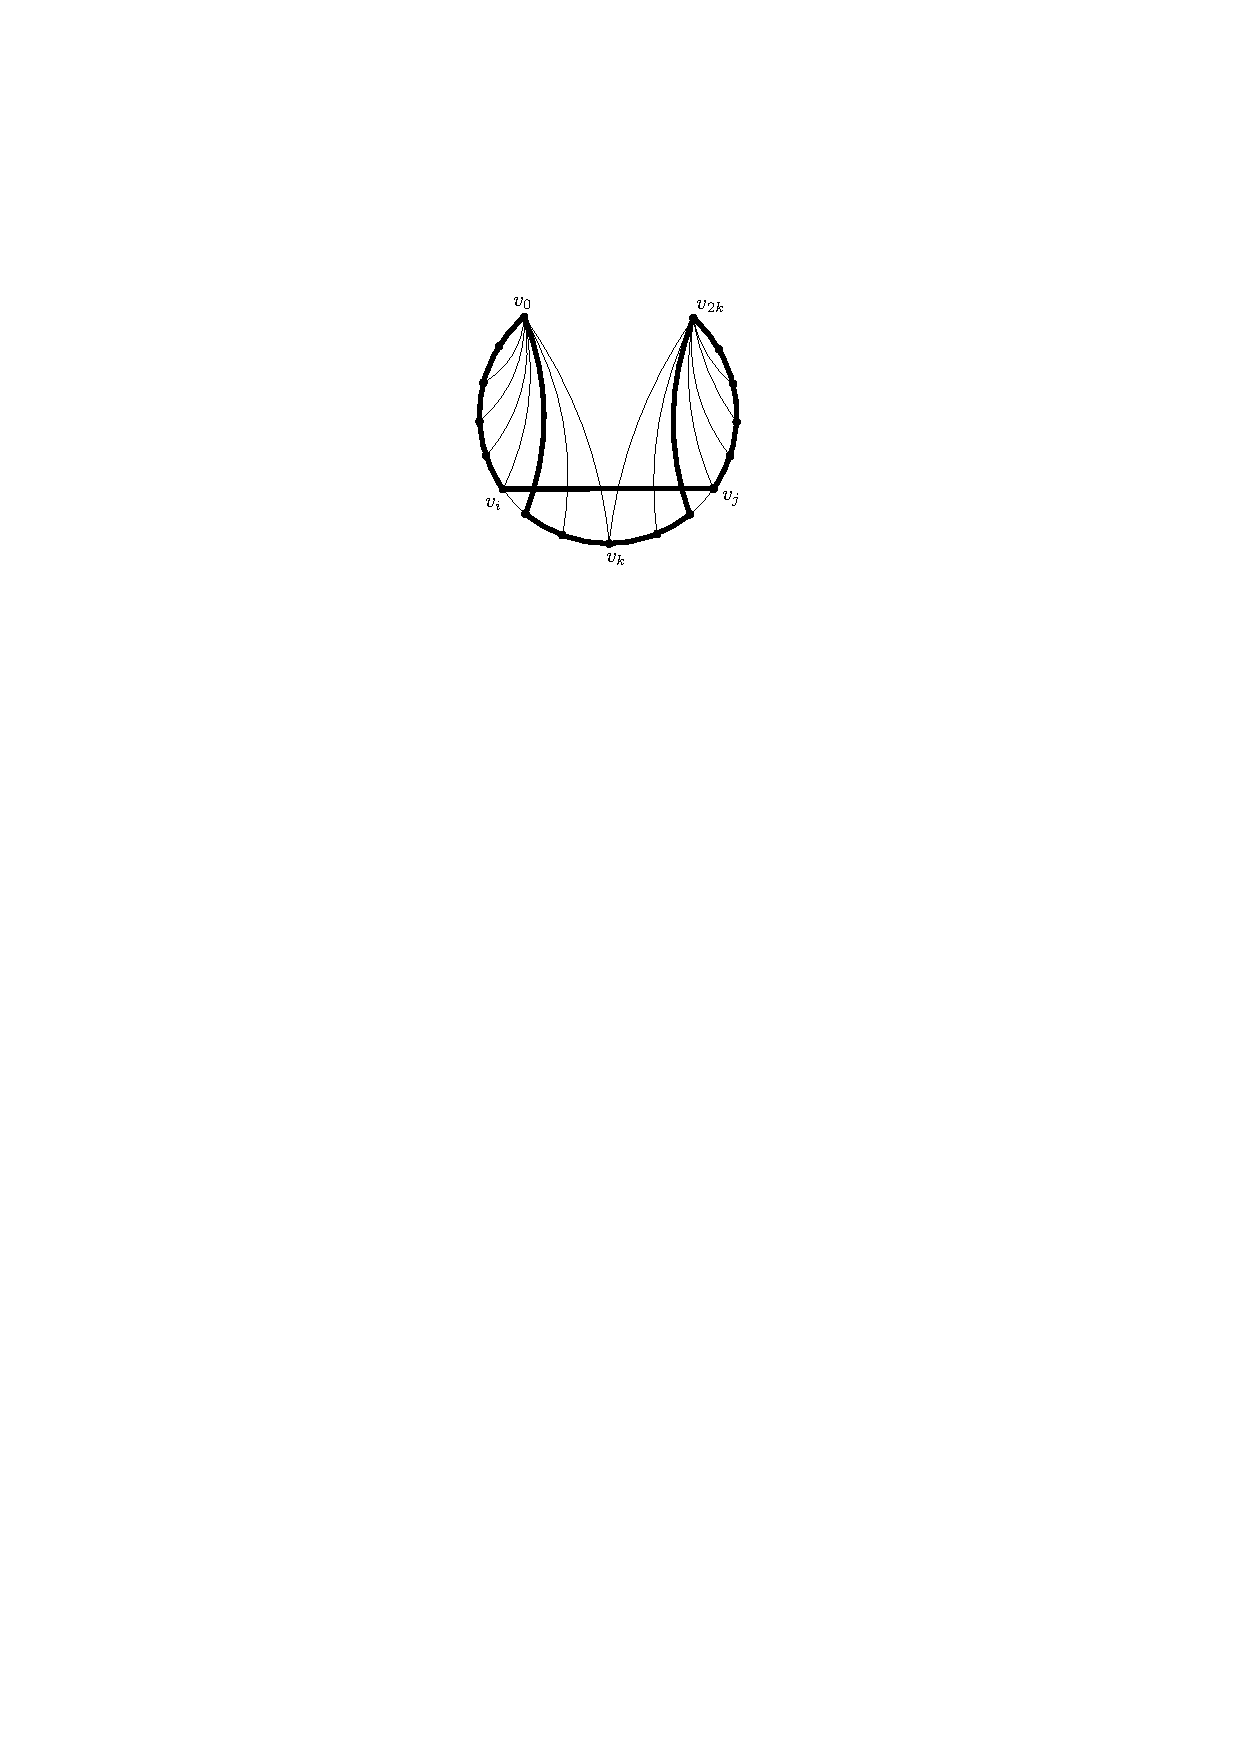
\includegraphics[width=7.5cm]{img/nash-williams2.pdf}
\caption{Případ (i)}
\label{dk:nw-i}
\end{subfigure}
\hfill
\begin{subfigure}{7.4cm}
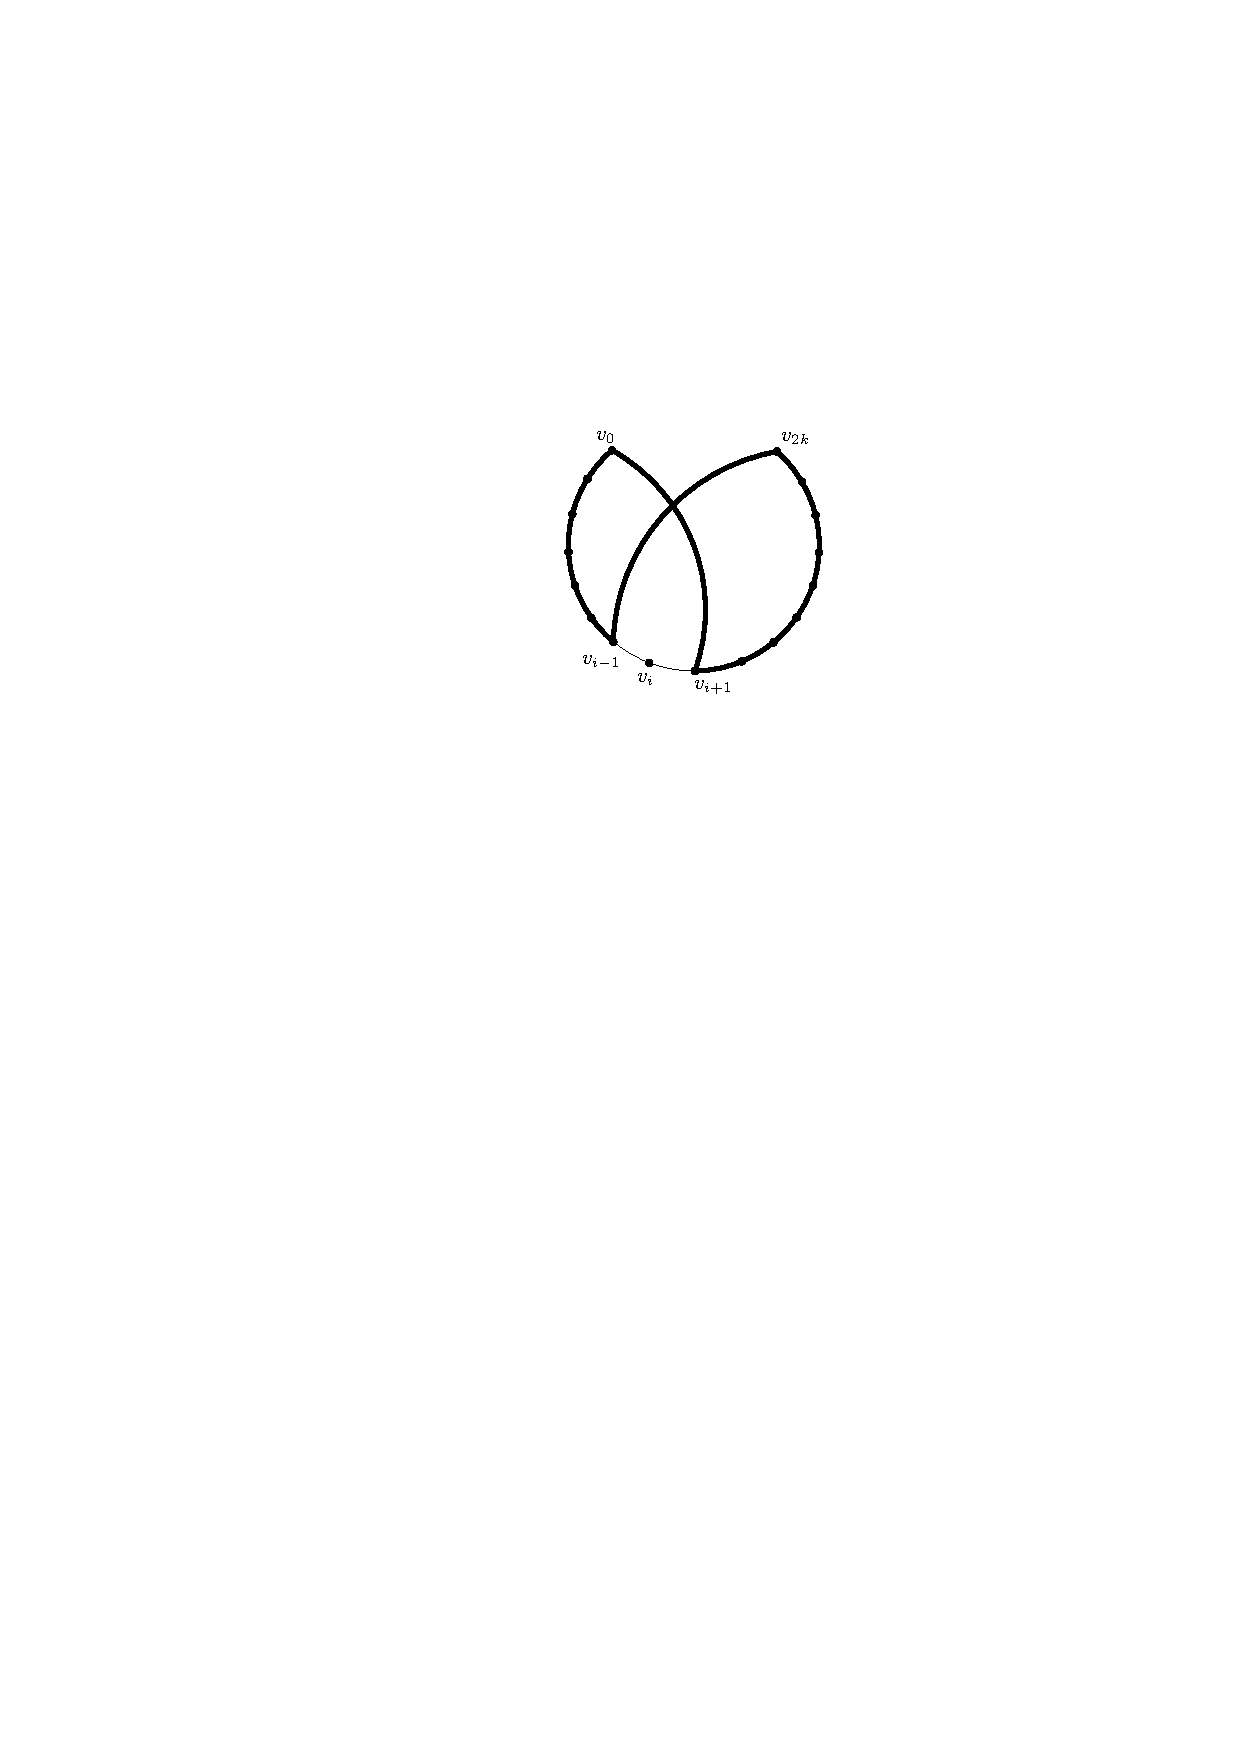
\includegraphics[width=7.5cm]{img/nash-williams3.pdf}
\caption{Případ (ii)}
\label{dk:nw-ii}
\end{subfigure}
\caption{Netriviální případy}
\end{figure}

